\documentclass[10pt, a4paper]{article}
\usepackage{graphicx} 
\usepackage{listings}
\usepackage{xcolor} 
\usepackage[table]{xcolor} 
\usepackage{amsmath}
\usepackage{amssymb}
\usepackage{wrapfig}
\usepackage{parskip}
\usepackage{float}
\usepackage{hyperref}
\usepackage[utf8]{inputenc}
\usepackage[T1]{fontenc}
\usepackage{siunitx}
\sisetup{output-decimal-marker = {,}}
\usepackage[swedish]{babel}
\usepackage{array}
\usepackage{adjustbox}
\usepackage[margin=2.5 cm]{geometry}
\usepackage{appendix}
\usepackage{csquotes}
\usepackage{comment}
\usepackage[
    sorting=none
]{biblatex}
\usepackage{titling}

\addbibresource{references.bib}

\lstdefinestyle{mypython}{
    language=Python,
    basicstyle=\ttfamily\small,
    backgroundcolor=\color{gray!10},
    keywordstyle=\color{blue}\bfseries,
    %stringstyle=\color{orange!85!black},
    commentstyle=\color{green!50!black},
    numberstyle=\tiny,
    numbers=left,
    stepnumber=1,
    numbersep=8pt,
    showstringspaces=false,
    frame=single,
    breaklines=true,
    breakatwhitespace=true,
    tabsize=4,
    morekeywords={self},  % Lägg till fler Python-nyckelord om nödvändigt
    literate={ö}{{\"o}}1 {å}{{\aa}}1 {ä}{{\"a}}1 {\\}{{\textbackslash}}1,
    }
    
\begin{document}

\pagenumbering{arabic}
\thispagestyle{empty}
\begin{center}
{\huge\bf Förstudie - Kvantfysik:\\}
{\Large\bf Studier av atomära spektrum
}
\end{center}
\vspace{1.0cm}
\begin{center}
Julius Berg (juliusbe), Benjamin Johansson (benjjoh), \par
Program: Teknisk fysik. \par
Kurs: TIF097 - Experimentell fysik 2.
\end{center}
\vspace{1.0cm}
\centerline{\bf Sammandrag}
 
\newpage
\tableofcontents
\newpage

\section{Inledning}

Alla grundämnen interagerar på olika sätt med elektromagnetisk strålning.
Detta sker både via absorption, då en elektron absorberar en foton och ökar i energi, eller emission, 
då en elektron minskar i energi och emitterar en foton med motsvarande energi.
Denna växelverkan sker dock endast vid specifika frekvenser, då elektroner i en atom endast kan existera
på specifika energinivåer.
När en elektron övergår från en energinivå till en energinivå med lägre energi frigörs därmed en foton som har en våglängd som ges av energiskillnaden mellan nivåerna.
Detta ger upphov till fotoner med en bestämd våglängd, så kallade spektrallinjer.

Eftersom olika grundämnen har olika elektronstrukturer har varje ämne en unik uppsättning möjliga energiövergångar.
Detta innebär att specifika grundämnen producerar unika uppsättningar av spektrallinjer.
Denna unika uppsättning fungerar som ett fingeravtryck för det specifika grundämnet, och detta faktum är mycket viktigt inom till exempel astronomi, 
där emissionsspektrum används för att bestämma vilka grundämnen och molekyler som finns i exoplaneters atmosfärer.

Syftet med denna studie är att för ett bestämt grundämne bestämma emissionsspektrum och utifrån detta emissionsspektrum konstruera grundämnets energinivådiagram.

\section{Teori}
En atoms energinivåer definieras av kombinationer av 4 kvanttal.
Dessa kvanttal kan tillsammans beskriva elektronkonfigurationen i en atom, och varje kombination av kvanttal motsvaras av en energinivå.
Kvanttalen är huvudkvanttalet $n$, bankvanttalet $l$, det magnetiska kvanttalet $m$ och spinnkvanttalet $s$.

Huvudkvanttalet $n$ relaterar till elektronens energi, och är ett naturligt tal. 
I Bohrs atommodell, som kännetecknas av en kärna och elektroner som cirkulerar i skal på bestämda avstånd från kärnan, är $n$ det enda kvanttalet.
Elektronens energi blir i det fallet 
\begin{equation}
    E_n = - \frac{me^4 Z^2}{8\varepsilon_0^2 h^2 n^2} = -Rhc_0\frac{Z^2}{n^2} 
\end{equation}
är m är systemets reducerade massa ($\approx m_e$), $e$ är elementarladdningen, $Z$ är antalet protoner i kärnan, $\varepsilon_0$ är permittiviteten i vakuum, 
$h$ är plancks konstant, $n$ är kvanttalet, $R$ är Rydbergs konstant och $c_0$ är ljusets hastighet i vakuum.
En schematisk bild av Bohrs atommodell visas nedan i figur \ref{fig:Bohr_atom_model}.

\begin{figure}[ht]
    \centering
    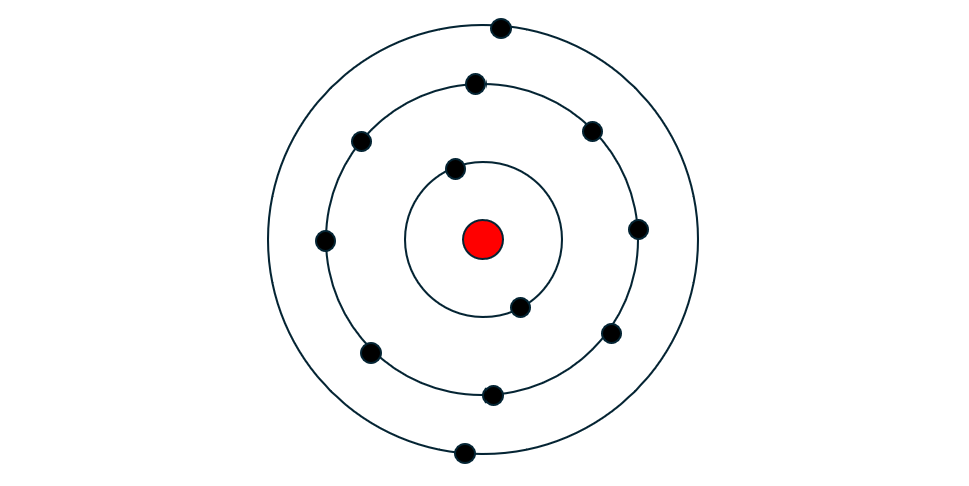
\includegraphics[width=0.5\linewidth]{../Bilder/Bohr_atom_model.png}
    \caption{\textit{Bohrs atommodell. Modellen utgår ifrån en positivt laddad kärna runt vilken det cirkulerar 
    flera negativt laddade elektroner. Elektronerna cirkulerar runt kärnan på bestämda avstånd, så kallade skal,
    som motsvaras av huvudkvanttalet $n$. Bohrs atommodell tar inte hänsyn till övriga kvanttal.}}
    \label{fig:Bohr_atom_model}
\end{figure}

Bohrs atommodell tar dock inte hänsyn till övriga kvanttal.
Bankvanttalet $l$ relaterar till elektronens rörelsemängdsmoment och är likt huvudkvanttalet $n$ ett positivt heltal.
Bankvanttalet $l$ är dock strikt mindre än $n$, vilket innebär att för varje ''skal'' $n$ finns det $n-1$ underskal relaterade till kvanttalet $l$.
Dessa underskal benämns enligt konvention med bokstäver istället för siffror, så de första 4 underskalen kallas s, p, d och f istället för 1, 2, 3 och 4.

Dessutom förekommer det magnetiska kvanttalet $m$, som beskriver bankvanttalets projektion på en given axel.
$m$ är även det ett heltal med möjliga värden mellan $-l \rightarrow l$.
Avslutningsvis finns även spinnkvanttalet $s$, där elektronen kan ha spinn $\frac{1}{2}$ (spinn upp) eller spinn $-\frac{1}{2}$ (spinn ned).

Kombinationer av dessa kvanttal relaterar till en viss energinivå, och när en elektron går från ett kvanttillstånd till ett annat kvanttillstånd måste den tillföras
eller avge energi så att dess nya energi stämmer med energin för det givna kvanttillståndet.
Denna energitillförsel sker ofta via samverkan med fotoner.
En foton har en energi som är linjärt proportionerlig mot frekvensen enligt sambandet 

\begin{equation}
    E = hf = h\frac{c_0}{\lambda},
    \label{eq:energi-våglängd-relation}
\end{equation}

där $E$ är energin, $f$ är frekvensen och $\lambda$ är våglängden.
När en elektron går från en högre energinivå $E_i$ till en lägre energinivå $E_f$ kommer den att avge en foton med energin 
\begin{equation}
    E = E_{i} - E_f.
    \label{eq:energiskillnad}
\end{equation}
Eftersom energinivåerna i atomen är specifika kommer också alla energiskillnader mellan nivåer att vara specifika.
Detta innebär att atomen kommer sända ut ett spektrum av fotoner med diskreta frekvenser,
vilket ger upphov till ett linjespektrum där varje spektrallinje motsvarar en övergång mellan 2 energitillstånd.
Figur \ref{fig:Exempel_emissionsspektra} visar ett simulerat emissionsspektrum där energiövergångarna emitterar fotoner med våglängder 450, 600 och 720 nm.

\begin{figure}[H]
    \centering
    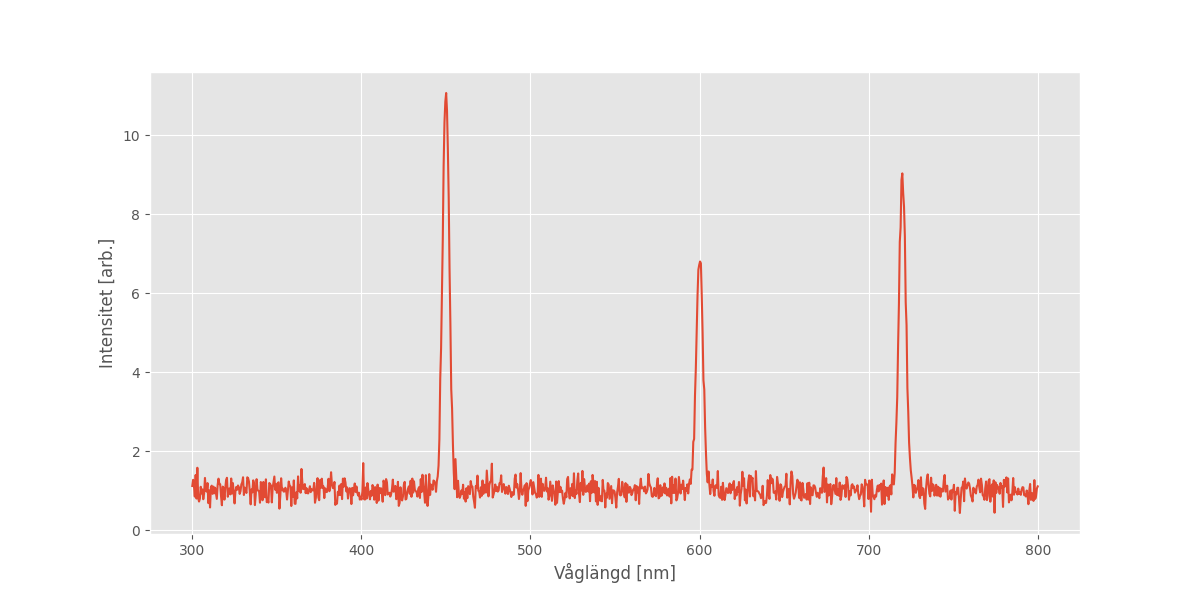
\includegraphics[width=0.7\textwidth]{../Bilder/Exempel_emissionsspektra.png}
    \caption{\textit{Simulerat emissionsspektrum. Figuren visar hur ett fiktivt grundämne emitterar fotoner med energier som
    motsvarar våglängderna 450, 600 och 720 nm.}}
    \label{fig:Exempel_emissionsspektra}
\end{figure}

Alla energiövergångar är dock inte tillåtna, utan bestäms av så kallade urvalsregler, vilka bestämmer vilka övergångar som är tillåtna.
För elektriska dipolövergångar, som dominerar atomära spektrum, gäller till exempel urvalsregeln
\begin{equation}
    \Delta l = \pm 1.
\end{equation}
Detta skapar en karta över möjliga energiövergångar, vilket gör det möjligt att konstruera så kallade energinivådiagram.
Dessa diagram visar grafiskt vilka energiövergångar som är tillåtna.
Figur \ref{fig:energinivådiagram_väte} visar energinivådiagrammet för väte för de första 4 huvudkvanttalen $n$.
Värt att notera är att inga övergångar sker mellan tillstånd med samma bankvanttal $l$.

\begin{figure}[ht]
    \centering
    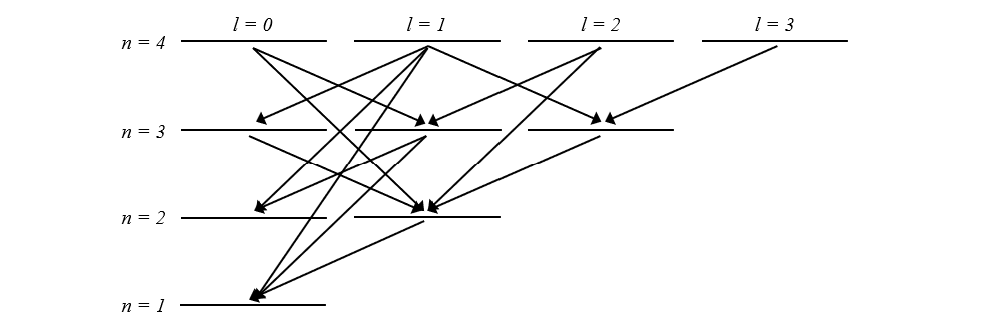
\includegraphics[width=0.7\textwidth]{../Bilder/energinivådiagram_väte.png}
    \caption{\textit{Energinivådiagram för de första 4 huvudkvanttalen av väte. Noterbart är att samtliga övergångar 
    följer urvalsregeln $\Delta l = \pm 1$. }}
    \label{fig:energinivådiagram_väte}
\end{figure}


\section{Metod}
\subsection{Försöksuppställning}
Uppställningen förväntas använda spektrumetern SPEX 270M, ett Hamamatsu R375 fotomultiplikatorrör, en Keithley 485 picoamperemeter
och en ljuskälla, enligt figur \ref{fig:Försöksuppställning}. Ljuskällan exciterar ett grundämne som vid deexcitation utstrålar ljus. 
\begin{figure}[H]
    \centering
    
\includegraphics[width=1\textwidth]{../Bilder/SPEX_270M.jpg}
    \caption{\textit{Den försöksuppställning som förväntas användas under laborationen. En ljuskälla från det exciterade ämnet 
    lyser in i en spektrumeter och förstärks med en fotomultiplikator. Signalen från fotomultiplikatorn mäts med en picoamperemeter.
    Hela uppställningen styrs via LabVIEW.}}
    \label{fig:Försöksuppställning}
\end{figure}
\subsection{Genomförande}
Då ljuskällan lyser in i spektrumetern kan en enskild våglängd väljas genom att justera gittrets position med en inre motor. Den monokroma strålen förstärks
i fotomultiplikatorröret och översätts till en elektrisk signal som kan mätas med picoamperemetern. Genom att justera vilken våglängd som väljs
i spektrometern och dokumentera strömstyrkan som mäts med amperemetern kan strömmens beroende på våglängden bestämmas. Ett emissionsspektrum kan 
sedan bildas genom att plotta strömmen mot våglängden. Både spektrumetern och picoamperemetern
förväntas styras via en egenskriven LabVIEW-kod, se appendix \ref{appendix:Labview}.

Från emissionsspektrumet kan sedan ett energinivådiagram konstrueras genom att finna centrum på spektrumets toppar och använda 
ekvationerna \ref{eq:energiskillnad} och \ref{eq:energi-våglängd-relation}.

\section{Förväntade resultat}
Det exakta emissionsspektrumet kan inte bestämmas utan att veta vilket grundämne som ska undersökas. Däremot kommer spektrumet anta ett generiskt utseende enligt figur \ref{fig:Exempel_emissionsspektra}.
Det förväntas finnas diskreta toppar som påvisar de våglängder ämnet emitterar. Energinivådiagrammet förväntas även kunna konstrueras från emissionsspektrumet.
\section{Diskussion}

% \newpage
% \printbibliography
\appendix
\newpage
\section{LabVIEW-kod}
\label{appendix:Labview}
Under laborationen förväntas ett egenskrivet LabVIEW-programm användas. Blockdiagrammet till detta program visas nedan i figur \ref{fig:LabVIEW-kod}.
\begin{figure}[H]
    \centering
    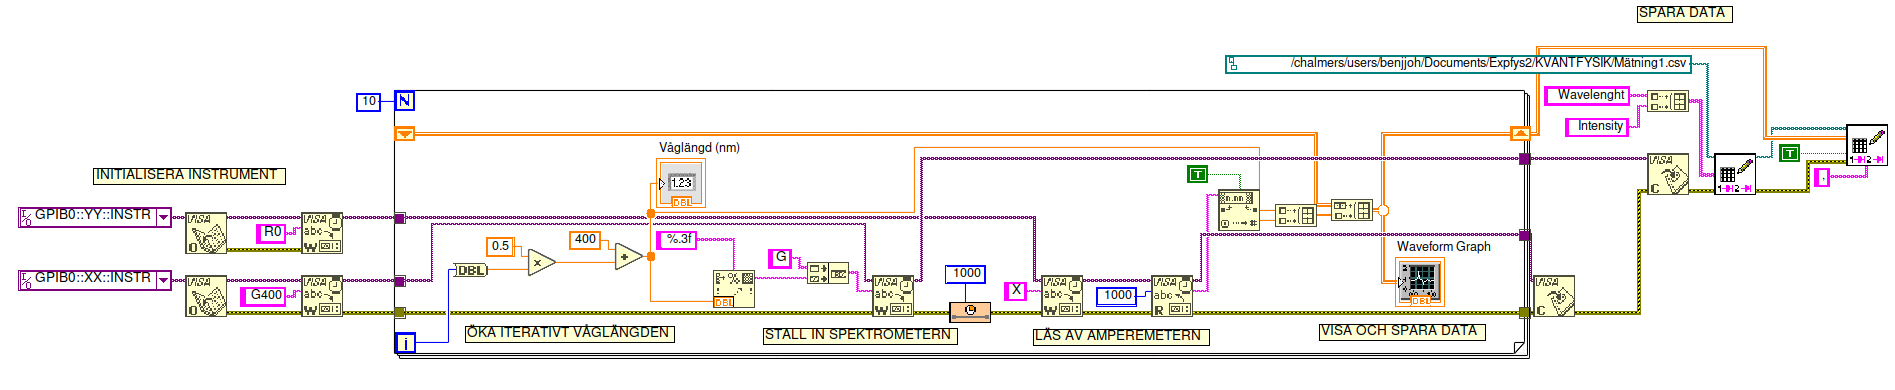
\includegraphics[width=1.25\linewidth, angle = -90]{../Bilder/Kvant Labview-bild.png}
    \caption{\textit{Den LabVIEW-kod som förväntas användas under laborationen. Först initialiseras spektrumetern och amperemetern.
    Sedan väljs vilken våglängd som spektrumetern ska låta igenom och strömmen från amperemetern sparas tillsammans med våglängden.
    Till sist sparas en .csv fil med våglängder och den ström som mäts vilket tillsammans bildar kan plottas till en intensitetsfördelning.}}
    \label{fig:LabVIEW-kod}
\end{figure}

\end{document}